\documentclass[twoside]{book}

% Packages required by doxygen
\usepackage{fixltx2e}
\usepackage{calc}
\usepackage{doxygen}
\usepackage[export]{adjustbox} % also loads graphicx
\usepackage{graphicx}
\usepackage[utf8]{inputenc}
\usepackage{makeidx}
\usepackage{multicol}
\usepackage{multirow}
\PassOptionsToPackage{warn}{textcomp}
\usepackage{textcomp}
\usepackage[nointegrals]{wasysym}
\usepackage[table]{xcolor}

% Font selection
\usepackage[T1]{fontenc}
\usepackage[scaled=.90]{helvet}
\usepackage{courier}
\usepackage{amssymb}
\usepackage{sectsty}
\renewcommand{\familydefault}{\sfdefault}
\allsectionsfont{%
  \fontseries{bc}\selectfont%
  \color{darkgray}%
}
\renewcommand{\DoxyLabelFont}{%
  \fontseries{bc}\selectfont%
  \color{darkgray}%
}
\newcommand{\+}{\discretionary{\mbox{\scriptsize$\hookleftarrow$}}{}{}}

% Page & text layout
\usepackage{geometry}
\geometry{%
  a4paper,%
  top=2.5cm,%
  bottom=2.5cm,%
  left=2.5cm,%
  right=2.5cm%
}
\tolerance=750
\hfuzz=15pt
\hbadness=750
\setlength{\emergencystretch}{15pt}
\setlength{\parindent}{0cm}
\setlength{\parskip}{3ex plus 2ex minus 2ex}
\makeatletter
\renewcommand{\paragraph}{%
  \@startsection{paragraph}{4}{0ex}{-1.0ex}{1.0ex}{%
    \normalfont\normalsize\bfseries\SS@parafont%
  }%
}
\renewcommand{\subparagraph}{%
  \@startsection{subparagraph}{5}{0ex}{-1.0ex}{1.0ex}{%
    \normalfont\normalsize\bfseries\SS@subparafont%
  }%
}
\makeatother

% Headers & footers
\usepackage{fancyhdr}
\pagestyle{fancyplain}
\fancyhead[LE]{\fancyplain{}{\bfseries\thepage}}
\fancyhead[CE]{\fancyplain{}{}}
\fancyhead[RE]{\fancyplain{}{\bfseries\leftmark}}
\fancyhead[LO]{\fancyplain{}{\bfseries\rightmark}}
\fancyhead[CO]{\fancyplain{}{}}
\fancyhead[RO]{\fancyplain{}{\bfseries\thepage}}
\fancyfoot[LE]{\fancyplain{}{}}
\fancyfoot[CE]{\fancyplain{}{}}
\fancyfoot[RE]{\fancyplain{}{\bfseries\scriptsize Generated by Doxygen }}
\fancyfoot[LO]{\fancyplain{}{\bfseries\scriptsize Generated by Doxygen }}
\fancyfoot[CO]{\fancyplain{}{}}
\fancyfoot[RO]{\fancyplain{}{}}
\renewcommand{\footrulewidth}{0.4pt}
\renewcommand{\chaptermark}[1]{%
  \markboth{#1}{}%
}
\renewcommand{\sectionmark}[1]{%
  \markright{\thesection\ #1}%
}

% Indices & bibliography
\usepackage{natbib}
\usepackage[titles]{tocloft}
\setcounter{tocdepth}{3}
\setcounter{secnumdepth}{5}
\makeindex

% Hyperlinks (required, but should be loaded last)
\usepackage{ifpdf}
\ifpdf
  \usepackage[pdftex,pagebackref=true]{hyperref}
\else
  \usepackage[ps2pdf,pagebackref=true]{hyperref}
\fi
\hypersetup{%
  colorlinks=true,%
  linkcolor=blue,%
  citecolor=blue,%
  unicode%
}

% Custom commands
\newcommand{\clearemptydoublepage}{%
  \newpage{\pagestyle{empty}\cleardoublepage}%
}

\usepackage{caption}
\captionsetup{labelsep=space,justification=centering,font={bf},singlelinecheck=off,skip=4pt,position=top}

%===== C O N T E N T S =====

\begin{document}

% Titlepage & ToC
\hypersetup{pageanchor=false,
             bookmarksnumbered=true,
             pdfencoding=unicode
            }
\pagenumbering{roman}
\begin{titlepage}
\vspace*{7cm}
\begin{center}%
{\Large My\+Project2 }\\
\vspace*{1cm}
{\large Generated by Doxygen 1.8.11}\\
\end{center}
\end{titlepage}
\clearemptydoublepage
\tableofcontents
\clearemptydoublepage
\pagenumbering{arabic}
\hypersetup{pageanchor=true}

%--- Begin generated contents ---
\chapter{Research Track I -\/ First Assignment}
\label{md_README}
\hypertarget{md_README}{}
In this repository you will find all the package required for the construction of a 2D robot whose goal is to achieve a target. Let me explain all the directory which are in this repository

\subsubsection*{my\+\_\+srv}

In this package you will find
\begin{DoxyItemize}
\item A subfolder /srv cointains Server1.\+srv -\/$>$ it contains all the paramaters that the Server1 required and the parameters that are returned.
\item A subfolder /src contains \hyperlink{random__server_8cpp}{random\+\_\+server.\+cpp} -\/$>$ the scope of this code is to provide a random position in a specific interval \mbox{[}-\/6.\+6\mbox{]}. Tha random position is given as input and the code returns it to /robot \+\_\+ controller node
\end{DoxyItemize}

\subsubsection*{robot}

In this package you will find
\begin{DoxyItemize}
\item A subfolder /src contains \hyperlink{robot__controller_8cpp}{robot\+\_\+controller.\+cpp} -\/$>$ it manages the motion of the robot and asks to the server a new target when the previous one is reached
\end{DoxyItemize}

\subsection*{How the node communicate to each other}



\subsection*{How to run the code\+:}


\begin{DoxyItemize}
\item As first step it is necessary to run a command to create the master 
\begin{DoxyCode}
1 roscore & 
\end{DoxyCode}

\item As second step run the simulation space with 
\begin{DoxyCode}
1 rosrun stage\_ros stageros $(rospack find assignment1)/world/exercise.world
\end{DoxyCode}

\item As third step in another shell use the command to run the server 
\begin{DoxyCode}
1 rosrun my\_srv random\_server
\end{DoxyCode}

\item As last step, in another shell, use the command to run the robot\+\_\+controller 
\begin{DoxyCode}
1 rosrun roboy robot\_controller
\end{DoxyCode}
 
\end{DoxyItemize}
\chapter{File Index}
\section{File List}
Here is a list of all files with brief descriptions\+:\begin{DoxyCompactList}
\item\contentsline{section}{my\+\_\+srv/src/\hyperlink{random__server_8cpp}{random\+\_\+server.\+cpp} }{\pageref{random__server_8cpp}}{}
\item\contentsline{section}{robot/src/\hyperlink{robot__controller_8cpp}{robot\+\_\+controller.\+cpp} }{\pageref{robot__controller_8cpp}}{}
\end{DoxyCompactList}

\chapter{File Documentation}
\hypertarget{random__server_8cpp}{}\section{my\+\_\+srv/src/random\+\_\+server.cpp File Reference}
\label{random__server_8cpp}\index{my\+\_\+srv/src/random\+\_\+server.\+cpp@{my\+\_\+srv/src/random\+\_\+server.\+cpp}}
{\ttfamily \#include \char`\"{}ros/ros.\+h\char`\"{}}\\*
{\ttfamily \#include \char`\"{}my\+\_\+srv/\+Server1.\+h\char`\"{}}\\*
{\ttfamily \#include $<$math.\+h$>$}\\*
Include dependency graph for random\+\_\+server.\+cpp\+:
\nopagebreak
\begin{figure}[H]
\begin{center}
\leavevmode
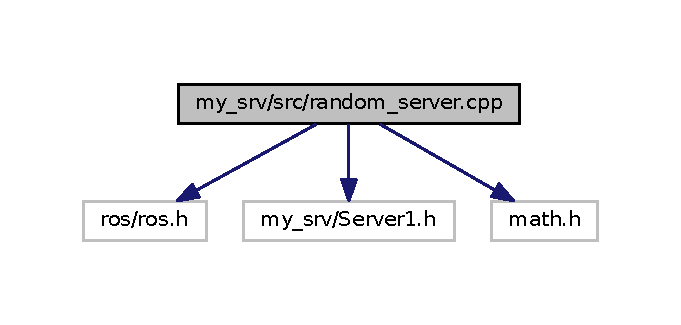
\includegraphics[width=327pt]{random__server_8cpp__incl}
\end{center}
\end{figure}
\subsection*{Functions}
\begin{DoxyCompactItemize}
\item 
bool \hyperlink{random__server_8cpp_a55eae18de3c41a40c7005b4faf39120d}{pos\+\_\+random} (my\+\_\+srv\+::\+Server1\+::\+Request \&req, my\+\_\+srv\+::\+Server1\+::\+Response \&res)
\item 
int \hyperlink{random__server_8cpp_a3c04138a5bfe5d72780bb7e82a18e627}{main} (int argc, char $\ast$$\ast$argv)
\end{DoxyCompactItemize}


\subsection{Function Documentation}
\index{random\+\_\+server.\+cpp@{random\+\_\+server.\+cpp}!main@{main}}
\index{main@{main}!random\+\_\+server.\+cpp@{random\+\_\+server.\+cpp}}
\subsubsection[{\texorpdfstring{main(int argc, char $\ast$$\ast$argv)}{main(int argc, char **argv)}}]{\setlength{\rightskip}{0pt plus 5cm}int main (
\begin{DoxyParamCaption}
\item[{int}]{argc, }
\item[{char $\ast$$\ast$}]{argv}
\end{DoxyParamCaption}
)}\hypertarget{random__server_8cpp_a3c04138a5bfe5d72780bb7e82a18e627}{}\label{random__server_8cpp_a3c04138a5bfe5d72780bb7e82a18e627}


Definition at line 15 of file random\+\_\+server.\+cpp.

\index{random\+\_\+server.\+cpp@{random\+\_\+server.\+cpp}!pos\+\_\+random@{pos\+\_\+random}}
\index{pos\+\_\+random@{pos\+\_\+random}!random\+\_\+server.\+cpp@{random\+\_\+server.\+cpp}}
\subsubsection[{\texorpdfstring{pos\+\_\+random(my\+\_\+srv\+::\+Server1\+::\+Request \&req, my\+\_\+srv\+::\+Server1\+::\+Response \&res)}{pos_random(my_srv::Server1::Request &req, my_srv::Server1::Response &res)}}]{\setlength{\rightskip}{0pt plus 5cm}bool pos\+\_\+random (
\begin{DoxyParamCaption}
\item[{my\+\_\+srv\+::\+Server1\+::\+Request \&}]{req, }
\item[{my\+\_\+srv\+::\+Server1\+::\+Response \&}]{res}
\end{DoxyParamCaption}
)}\hypertarget{random__server_8cpp_a55eae18de3c41a40c7005b4faf39120d}{}\label{random__server_8cpp_a55eae18de3c41a40c7005b4faf39120d}


Definition at line 7 of file random\+\_\+server.\+cpp.


\hypertarget{_r_e_a_d_m_e_8md}{}\section{R\+E\+A\+D\+M\+E.\+md File Reference}
\label{_r_e_a_d_m_e_8md}\index{R\+E\+A\+D\+M\+E.\+md@{R\+E\+A\+D\+M\+E.\+md}}

\hypertarget{robot__controller_8cpp}{}\section{robot/src/robot\+\_\+controller.cpp File Reference}
\label{robot__controller_8cpp}\index{robot/src/robot\+\_\+controller.\+cpp@{robot/src/robot\+\_\+controller.\+cpp}}
{\ttfamily \#include \char`\"{}ros/ros.\+h\char`\"{}}\\*
{\ttfamily \#include \char`\"{}geometry\+\_\+msgs/\+Twist.\+h\char`\"{}}\\*
{\ttfamily \#include \char`\"{}nav\+\_\+msgs/\+Odometry.\+h\char`\"{}}\\*
{\ttfamily \#include \char`\"{}my\+\_\+srv/\+Server1.\+h\char`\"{}}\\*
Include dependency graph for robot\+\_\+controller.\+cpp\+:
\nopagebreak
\begin{figure}[H]
\begin{center}
\leavevmode
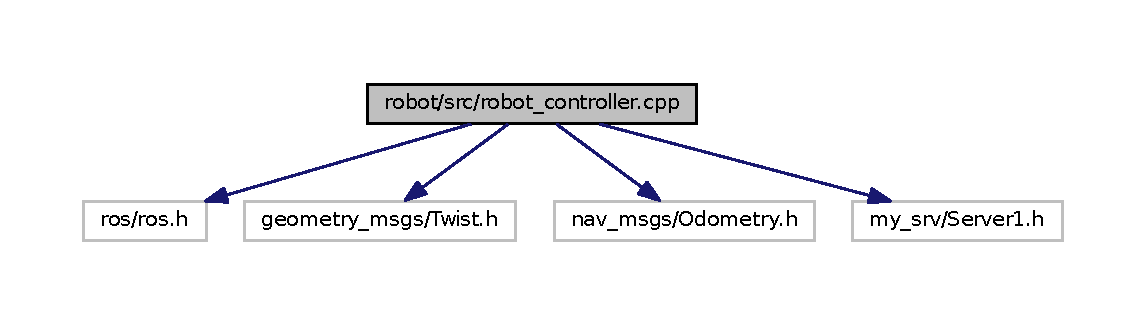
\includegraphics[width=350pt]{robot__controller_8cpp__incl}
\end{center}
\end{figure}
\subsection*{Functions}
\begin{DoxyCompactItemize}
\item 
void \hyperlink{robot__controller_8cpp_aab6e381bffc34921244a29ec0538ba64}{position\+Callback} (const nav\+\_\+msgs\+::\+Odometry\+::\+Const\+Ptr \&msg)
\item 
int \hyperlink{robot__controller_8cpp_a3c04138a5bfe5d72780bb7e82a18e627}{main} (int argc, char $\ast$$\ast$argv)
\end{DoxyCompactItemize}
\subsection*{Variables}
\begin{DoxyCompactItemize}
\item 
ros\+::\+Publisher \hyperlink{robot__controller_8cpp_a350594df3e8f6948c8462edfd41ce086}{pub}
\item 
ros\+::\+Service\+Client \hyperlink{robot__controller_8cpp_a17bcd065930a8a7f9f194078d9977268}{client}
\item 
my\+\_\+srv\+::\+Server1 \hyperlink{robot__controller_8cpp_a0f620f841aa4b0c612aedc7f0ecb2887}{rec\+\_\+pos}
\item 
float \hyperlink{robot__controller_8cpp_a2b38da70bc534912b1a64a4ef9d4685d}{x\+\_\+target} = 0
\item 
float \hyperlink{robot__controller_8cpp_a046bc8e8769567b4762db66344df6070}{y\+\_\+target} = 0
\end{DoxyCompactItemize}


\subsection{Function Documentation}
\index{robot\+\_\+controller.\+cpp@{robot\+\_\+controller.\+cpp}!main@{main}}
\index{main@{main}!robot\+\_\+controller.\+cpp@{robot\+\_\+controller.\+cpp}}
\subsubsection[{\texorpdfstring{main(int argc, char $\ast$$\ast$argv)}{main(int argc, char **argv)}}]{\setlength{\rightskip}{0pt plus 5cm}int main (
\begin{DoxyParamCaption}
\item[{int}]{argc, }
\item[{char $\ast$$\ast$}]{argv}
\end{DoxyParamCaption}
)}\hypertarget{robot__controller_8cpp_a3c04138a5bfe5d72780bb7e82a18e627}{}\label{robot__controller_8cpp_a3c04138a5bfe5d72780bb7e82a18e627}


Definition at line 48 of file robot\+\_\+controller.\+cpp.

\index{robot\+\_\+controller.\+cpp@{robot\+\_\+controller.\+cpp}!position\+Callback@{position\+Callback}}
\index{position\+Callback@{position\+Callback}!robot\+\_\+controller.\+cpp@{robot\+\_\+controller.\+cpp}}
\subsubsection[{\texorpdfstring{position\+Callback(const nav\+\_\+msgs\+::\+Odometry\+::\+Const\+Ptr \&msg)}{positionCallback(const nav_msgs::Odometry::ConstPtr &msg)}}]{\setlength{\rightskip}{0pt plus 5cm}void position\+Callback (
\begin{DoxyParamCaption}
\item[{const nav\+\_\+msgs\+::\+Odometry\+::\+Const\+Ptr \&}]{msg}
\end{DoxyParamCaption}
)}\hypertarget{robot__controller_8cpp_aab6e381bffc34921244a29ec0538ba64}{}\label{robot__controller_8cpp_aab6e381bffc34921244a29ec0538ba64}


Definition at line 20 of file robot\+\_\+controller.\+cpp.



\subsection{Variable Documentation}
\index{robot\+\_\+controller.\+cpp@{robot\+\_\+controller.\+cpp}!client@{client}}
\index{client@{client}!robot\+\_\+controller.\+cpp@{robot\+\_\+controller.\+cpp}}
\subsubsection[{\texorpdfstring{client}{client}}]{\setlength{\rightskip}{0pt plus 5cm}ros\+::\+Service\+Client client}\hypertarget{robot__controller_8cpp_a17bcd065930a8a7f9f194078d9977268}{}\label{robot__controller_8cpp_a17bcd065930a8a7f9f194078d9977268}


Definition at line 8 of file robot\+\_\+controller.\+cpp.

\index{robot\+\_\+controller.\+cpp@{robot\+\_\+controller.\+cpp}!pub@{pub}}
\index{pub@{pub}!robot\+\_\+controller.\+cpp@{robot\+\_\+controller.\+cpp}}
\subsubsection[{\texorpdfstring{pub}{pub}}]{\setlength{\rightskip}{0pt plus 5cm}ros\+::\+Publisher pub}\hypertarget{robot__controller_8cpp_a350594df3e8f6948c8462edfd41ce086}{}\label{robot__controller_8cpp_a350594df3e8f6948c8462edfd41ce086}


Definition at line 7 of file robot\+\_\+controller.\+cpp.

\index{robot\+\_\+controller.\+cpp@{robot\+\_\+controller.\+cpp}!rec\+\_\+pos@{rec\+\_\+pos}}
\index{rec\+\_\+pos@{rec\+\_\+pos}!robot\+\_\+controller.\+cpp@{robot\+\_\+controller.\+cpp}}
\subsubsection[{\texorpdfstring{rec\+\_\+pos}{rec_pos}}]{\setlength{\rightskip}{0pt plus 5cm}my\+\_\+srv\+::\+Server1 rec\+\_\+pos}\hypertarget{robot__controller_8cpp_a0f620f841aa4b0c612aedc7f0ecb2887}{}\label{robot__controller_8cpp_a0f620f841aa4b0c612aedc7f0ecb2887}


Definition at line 11 of file robot\+\_\+controller.\+cpp.

\index{robot\+\_\+controller.\+cpp@{robot\+\_\+controller.\+cpp}!x\+\_\+target@{x\+\_\+target}}
\index{x\+\_\+target@{x\+\_\+target}!robot\+\_\+controller.\+cpp@{robot\+\_\+controller.\+cpp}}
\subsubsection[{\texorpdfstring{x\+\_\+target}{x_target}}]{\setlength{\rightskip}{0pt plus 5cm}float x\+\_\+target = 0}\hypertarget{robot__controller_8cpp_a2b38da70bc534912b1a64a4ef9d4685d}{}\label{robot__controller_8cpp_a2b38da70bc534912b1a64a4ef9d4685d}


Definition at line 14 of file robot\+\_\+controller.\+cpp.

\index{robot\+\_\+controller.\+cpp@{robot\+\_\+controller.\+cpp}!y\+\_\+target@{y\+\_\+target}}
\index{y\+\_\+target@{y\+\_\+target}!robot\+\_\+controller.\+cpp@{robot\+\_\+controller.\+cpp}}
\subsubsection[{\texorpdfstring{y\+\_\+target}{y_target}}]{\setlength{\rightskip}{0pt plus 5cm}float y\+\_\+target = 0}\hypertarget{robot__controller_8cpp_a046bc8e8769567b4762db66344df6070}{}\label{robot__controller_8cpp_a046bc8e8769567b4762db66344df6070}


Definition at line 15 of file robot\+\_\+controller.\+cpp.


%--- End generated contents ---

% Index
\backmatter
\newpage
\phantomsection
\clearemptydoublepage
\addcontentsline{toc}{chapter}{Index}
\printindex

\end{document}
